\documentclass[11pt,aspectratio=43]{beamer}

\usepackage{amsmath,amssymb}
\usepackage{array}
\usepackage{booktabs}
\usepackage{graphicx}
\usepackage[numbers,sort&compress]{natbib}
\usepackage{xcolor}
\usepackage{tikz}
\usetikzlibrary{arrows.meta,positioning,shapes.geometric,calc}

\definecolor{accent}{HTML}{2E75B6}

\setbeameroption{hide notes}
\setbeamertemplate{navigation symbols}{}
\setbeamersize{text margin left=0.8cm,text margin right=0.8cm}

\setbeamercolor{normal text}{fg=black,bg=white}
\setbeamercolor{frametitle}{fg=black,bg=white}
\setbeamercolor{title}{fg=black}
\setbeamercolor{structure}{fg=black}
\setbeamercolor{alerted text}{fg=accent}
\setbeamercolor{block title}{fg=black,bg=black!10}
\setbeamercolor{block body}{fg=black,bg=black!3}
\setbeamercolor{itemize item}{fg=black}
\setbeamercolor{itemize subitem}{fg=black}

\setbeamerfont{title}{size=\normalsize,series=\bfseries}
\setbeamerfont{frametitle}{size=\normalsize,series=\bfseries}
\setbeamerfont{block title}{size=\normalsize,series=\bfseries}
\setbeamerfont{block body}{size=\normalsize}

\setbeamertemplate{footline}{%
  \leavevmode%
  \hbox{%
    \begin{beamercolorbox}[wd=\paperwidth,ht=2.8ex,dp=1.2ex,rightskip=0.8cm]{author in head/foot}%
      \insertframenumber
    \end{beamercolorbox}%
  }%
}

\title{Octopus CXL Memory Pooling: Data Augmentation, Training, and Reward Redesign}
\author{Pulak Mehrotra}
\date{March 2026}

\begin{document}

\begin{frame}[plain]
  \titlepage
\end{frame}

% =========================================================================
% EPISODE DIAGRAM
% =========================================================================

\begin{frame}{Each training episode replays one pod's VM arrivals as a sequence of allocation decisions.}
  \begin{center}
  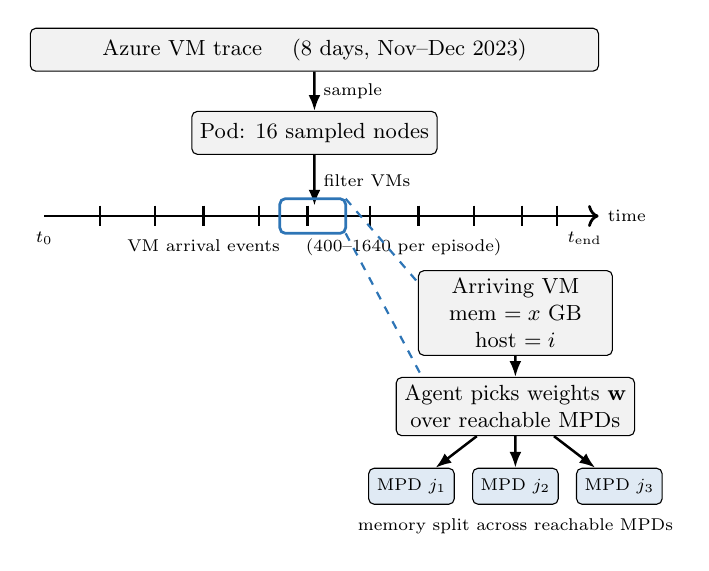
\begin{tikzpicture}[
      scale=0.88, transform shape,
      every node/.style={font=\small},
      box/.style={draw, rounded corners=2pt, fill=black!5,
                  minimum height=0.62cm, align=center},
      mpd/.style={draw, rounded corners=2pt, fill=accent!15,
                  minimum width=0.9cm, minimum height=0.52cm, align=center, font=\scriptsize},
      arr/.style={-{Latex[length=2mm]}, line width=0.9pt},
      darr/.style={{Latex[length=2mm]}-{Latex[length=2mm]}, line width=0.7pt, dashed}
  ]

    % --- Trace bar ---
    \node[box, minimum width=8.2cm] (trace) at (4.1, 3.8)
          {Azure VM trace \quad (8 days, Nov--Dec 2023)};

    % --- Pod sampling ---
    \node[box, minimum width=3.2cm] (pod) at (4.1, 2.6)
          {Pod: 16 sampled nodes};
    \draw[arr] (trace) -- (pod) node[midway, right, font=\scriptsize] {sample};

    % --- Timeline ---
    \draw[->, line width=1pt] (0.2, 1.4) -- (8.2, 1.4)
          node[right, font=\scriptsize] {time};
    \node[font=\scriptsize, anchor=north] at (0.2, 1.3) {$t_0$};
    \node[font=\scriptsize, anchor=north] at (8.0, 1.3) {$t_\text{end}$};

    % VM arrival ticks
    \foreach \x in {1.0, 1.8, 2.5, 3.3, 4.0, 4.9, 5.6, 6.4, 7.1, 7.6} {
      \draw[line width=0.8pt] (\x, 1.55) -- (\x, 1.25);
    }
    \node[font=\scriptsize] at (4.1, 0.95) {VM arrival events \quad (400--1640 per episode)};

    \draw[arr] (pod) -- (4.1, 1.55) node[midway, right, font=\scriptsize] {filter VMs};

    % --- Zoom box around one event ---
    \draw[accent, line width=1pt, rounded corners=2pt]
          (3.6, 1.65) rectangle (4.55, 1.15);
    \draw[accent, line width=0.8pt, dashed]
          (4.55, 1.65) -- (5.8, 0.2);
    \draw[accent, line width=0.8pt, dashed]
          (4.55, 1.15) -- (5.8, -1.2);

    % --- Decision box ---
    \node[box, minimum width=2.8cm] (event) at (7.0, -0.0)
          {Arriving VM\\mem $= x$ GB\\host $= i$};

    \node[box, minimum width=2.8cm] (agent) at (7.0, -1.35)
          {Agent picks weights $\mathbf{w}$\\over reachable MPDs};

    \draw[arr] (event) -- (agent);

    % MPD nodes
    \node[mpd] (m1) at (5.5, -2.5) {MPD $j_1$};
    \node[mpd] (m2) at (7.0, -2.5) {MPD $j_2$};
    \node[mpd] (m3) at (8.5, -2.5) {MPD $j_3$};
    \draw[arr] (agent) -- (m1);
    \draw[arr] (agent) -- (m2);
    \draw[arr] (agent) -- (m3);

    \node[font=\scriptsize, anchor=north] at (7.0, -2.85) {memory split across reachable MPDs};

  \end{tikzpicture}
  \end{center}
\end{frame}

% =========================================================================
% SLIDE 1: What does the training data look like?
% =========================================================================

\begin{frame}{The training data is ten Azure VM traces replayed as episode streams.}

  \begin{columns}[T,onlytextwidth]
    \column{0.48\textwidth}
      \begin{block}{Trace corpus}
        \begin{itemize}
          \item 10 production Azure VM traces; 8-day window (Nov--Dec 2023)
          \item Locations: Amsterdam, Bangalore, Dublin, London, Singapore, and others
          \item VM counts range from 23k (London) to 271k (Louisville) per trace
        \end{itemize}
      \end{block}

    \column{0.52\textwidth}
      \begin{block}{Episode structure}
        \begin{itemize}
          \item Per episode: sample a \emph{pod} of 16 nodes from one trace
          \item Each VM arrival becomes one allocation event: \texttt{(tick, host, mem\,MB, dealloc\_tick)}
          \item Episode length: 400--1640 events depending on trace and pod
        \end{itemize}
      \end{block}
  \end{columns}

\end{frame}

\begin{frame}{The environment reads one memory field per VM; data quality artifacts are filtered before training.}

  \begin{columns}[T,onlytextwidth]
    \column{0.52\textwidth}
      \begin{block}{Key data signal: \texttt{rss[1]}}
        The environment reads one field per VM: static memory allocation in MB.
        Values cluster at powers of two (512, 1024, 2048\,MB, \ldots) because
        Azure VMs are provisioned in standard SKU sizes.

        \vspace{0.3em}
        Time-series utilisation fields (\texttt{avg\_mem\_ts}, \texttt{max\_mem\_ts})
        exist in the trace but are not yet consumed by the environment.
      \end{block}
    \column{0.48\textwidth}
      \begin{block}{Data quality}
        \begin{itemize}
          \item 14--19\,\% of VMs carry a sentinel \texttt{end\_time}
                (\texttt{datetime(2020,1,1)}), giving a negative computed
                lifetime. All are caught and removed by the HOTFIX filter.
          \item 4--14\,\% have zero lifetime (\texttt{start} $=$ \texttt{end}).
          \item At the default scale, \textbf{81\,\%} of VMs survive into the
                episode event stream.
        \end{itemize}
      \end{block}
  \end{columns}

\end{frame}

% =========================================================================
% SLIDE 2: How can we augment this?
% =========================================================================

\begin{frame}{Episode-level augmentation generates diverse operating regimes without breaking SKU structure.}

  \begin{columns}[T,onlytextwidth]
    \column{0.48\textwidth}
      \begin{block}{Why augmentation is necessary}
        With one trace and one fixed pod assignment, the policy memorizes a single
        datacenter's workload pattern and fails to generalize.
        Augmentation is the standard remedy for train--eval distribution mismatch
        \cite{tobin2017domain,laskin2020rad}.
      \end{block}

    \column{0.52\textwidth}
      \begin{block}{Why episode-level, not per-VM}
        \texttt{rss[1]} is a discrete SKU variable: values cluster at powers of two
        (512, 1024, 2048\,MB, \ldots).
        Per-VM scaling creates synthetic memory sizes that do not exist in production.

        \vspace{0.3em}
        The correct unit is the \emph{episode}: one scale factor $s$ applied uniformly
        to all VMs, preserving relative sizes.
        This is the same principle as domain randomization \cite{tobin2017domain}:
        randomize environment conditions, not individual samples.
      \end{block}
  \end{columns}

\end{frame}

% =========================================================================
% SLIDE 3: Augmentation knobs
% =========================================================================

\begin{frame}{Six augmentation knobs span trace diversity, memory scale, and topology perturbation.}

  \begin{center}
  \small
  \begin{tabular}{lll}
    \toprule
    \textbf{Knob} & \textbf{Range / values} & \textbf{Priority} \\
    \midrule
    Multi-trace sampling    & 7 training traces (7/1/2 split)        & P0 (always on) \\
    Pod seed randomization  & $[0,\; 2^{31})$ per episode             & P0 (always on) \\
    Memory scale $s$        & $\mathcal{U}_\triangle(0.7, 1.0, 1.2)$ & P0 (always on) \\
    \midrule
    Link failures           & $\{0, 0.01, 0.02, 0.03, 0.05\}$       & P1 (ablation) \\
    Per-VM noise            & $\sigma \leq 0.03$ (lognormal)         & P1 (ablation) \\
    Arrival jitter          & $\pm 1$ tick                           & P1 (ablation) \\
    \midrule
    Lifetime perturbation   & fraction $\leq 0.05$                   & P2 (optional) \\
    \bottomrule
  \end{tabular}
  \end{center}

  \vspace{0.6em}

  \textbf{Train / validation / test split.}
  7 traces are used for training (with full augmentation), 1 for validation (no augmentation),
  and 2 for final held-out test (no augmentation, used once).
  Augmentation is \emph{never} applied during evaluation so that metrics reflect real trace
  distributions.

  \vspace{0.4em}

  % \textbf{Validity guards.}
  % Each augmented episode must satisfy: (1) pass the HOTFIX filter after scaling,
  % (2) contain at least 100 events, (3) leave every host connected to at least one MPD
  % after link injection.
  % If any guard fails, augmentation parameters are resampled for that episode.

\end{frame}

% =========================================================================
% ROLLOUT / RESET DIAGRAM
% =========================================================================

\begin{frame}{A rollout collects steps within one episode; a reset ends the episode and starts the next.}
  \begin{center}
  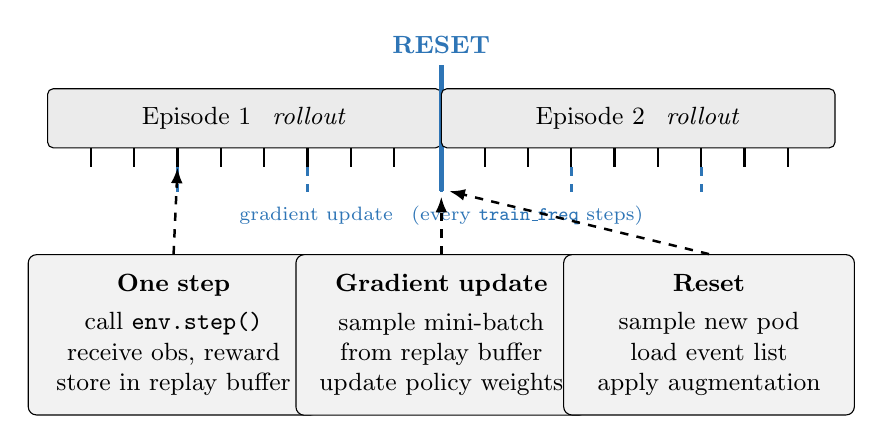
\begin{tikzpicture}[
      every node/.style={font=\small},
      arr/.style={-{Latex[length=2mm]}, line width=0.9pt},
      ann/.style={draw, rounded corners=3pt, fill=black!5,
                  align=center, inner sep=7pt}
  ]

    % ---- Episode 1 bar ----
    \draw[fill=black!8, draw=black, rounded corners=2pt]
          (0, 0) rectangle (5.0, 0.75);
    \node at (2.5, 0.375) {Episode 1 \enspace \textit{\small rollout}};

    % ---- Step ticks (episode 1) ----
    \foreach \x in {0.55, 1.1, 1.65, 2.2, 2.75, 3.3, 3.85, 4.4} {
      \draw[line width=0.8pt] (\x, 0) -- (\x, -0.25);
    }

    % ---- RESET marker ----
    \draw[line width=1.8pt, accent] (5.0, 1.05) -- (5.0, -0.55);
    \node[font=\small\bfseries, text=accent] at (5.0, 1.3) {RESET};

    % ---- Episode 2 bar ----
    \draw[fill=black!8, draw=black, rounded corners=2pt]
          (5.0, 0) rectangle (10.0, 0.75);
    \node at (7.5, 0.375) {Episode 2 \enspace \textit{\small rollout}};

    % ---- Step ticks (episode 2) ----
    \foreach \x in {5.55, 6.1, 6.65, 7.2, 7.75, 8.3, 8.85, 9.4} {
      \draw[line width=0.8pt] (\x, 0) -- (\x, -0.25);
    }

    % ---- Gradient update ticks ----
    \foreach \x in {1.65, 3.3, 5.0, 6.65, 8.3} {
      \draw[line width=1.0pt, accent, dashed] (\x, -0.25) -- (\x, -0.6);
    }
    \node[font=\scriptsize, text=accent, anchor=north] at (5.0, -0.62)
          {gradient update \enspace (every \texttt{train\_freq} steps)};

    % ---- Annotation boxes ----
    \node[ann, text width=3.2cm, anchor=north] (stepbox) at (1.6, -1.35) {%
      \textbf{One step}\\[3pt]
      call \texttt{env.step()}\\
      receive obs, reward\\
      store in replay buffer};

    \node[ann, text width=3.2cm, anchor=north] (gradbox) at (5.0, -1.35) {%
      \textbf{Gradient update}\\[3pt]
      sample mini-batch\\
      from replay buffer\\
      update policy weights};

    \node[ann, text width=3.2cm, anchor=north] (resetbox) at (8.4, -1.35) {%
      \textbf{Reset}\\[3pt]
      sample new pod\\
      load event list\\
      apply augmentation};

    % Arrows
    \draw[arr, dashed] (stepbox.north) -- (1.65, -0.25);
    \draw[arr, dashed] (gradbox.north) -- (5.0, -0.62);
    \draw[arr, dashed] (resetbox.north) -- (5.1, -0.55);

  \end{tikzpicture}
  \end{center}

\end{frame}

% =========================================================================
% SLIDE 4: Previous system and bottlenecks
% =========================================================================

\begin{frame}{The previous training setup had three compounding bottlenecks.}

  \begin{columns}[T,onlytextwidth]
    \column{0.50\textwidth}
      \begin{block}{Throughput bottlenecks}
        \small
        \begin{itemize}
          \item \textbf{Serial rollout.} \texttt{DummyVecEnv($N=1$)};
                $\sim$46 steps/sec; GPU utilization ${<}10\,\%$.
          \item \textbf{Slow reset.} Each episode start runs an
                $O(|\text{VMs}|)$ filter-and-sort pass; $\sim$120\,ms.
          \item \textbf{Few gradient updates.} 1M steps at
                \texttt{train\_freq}$=16$ yields only $\sim$62k
                policy updates. Standard vs.\ fast config:
                no measurable difference in final policy quality.
        \end{itemize}
      \end{block}

    \column{0.50\textwidth}
      \begin{block}{Policy failure: 20$\times$ MPD imbalance}
        \small
        \begin{itemize}
          \item SAC collapsed all load onto one or two MPDs;
                max/min load ratio $\sim$20$\times$.
          \item Greedy (na\"ive first-fit) outperformed SAC
                on held-out evaluation.
          \item Root cause: state and reward design, not
                training budget. The policy converged early
                to a degenerate solution because the reward
                gave signal only on the single worst MPD.
        \end{itemize}
      \end{block}
  \end{columns}

\end{frame}

% =========================================================================
% SLIDE 5: Rollout optimization
% =========================================================================

\begin{frame}{Parallel environments and a precomputed event cache deliver a 26$\times$ throughput gain.}

  \small
  \begin{tabular}{@{}p{0.46\textwidth}p{0.54\textwidth}@{}}
    \textbf{Fix 1: \texttt{SubprocVecEnv($N=32$)}} &
    \textbf{Fix 2: Precomputed event cache} \\
    $N$ workers run in parallel; observations batched into one GPU kernel per step. &
    Pod event lists built offline. \texttt{env.reset()} becomes $O(1)$. Reset: 120\,ms $\to$ 7\,ms. \\
  \end{tabular}

  \vspace{0.3em}

  \begin{center}
  \small
  \begin{tabular}{lrr}
    \toprule
    \textbf{Configuration} & \textbf{Steps / sec} & \textbf{Speedup} \\
    \midrule
    Baseline \texttt{DummyVecEnv} ($N=1$) & 46   & 1$\times$ \\
    \texttt{SubprocVecEnv} $N=4$          & 191  & 4.1$\times$ \\
    \texttt{SubprocVecEnv} $N=8$          & 369  & 8.0$\times$ \\
    \texttt{SubprocVecEnv} $N=16$         & 657  & 14.2$\times$ \\
    \texttt{SubprocVecEnv} $N=32$         & 1221 & \textbf{26.5$\times$} \\
    \bottomrule
  \end{tabular}
  \end{center}

  \vspace{0.2em}
  \begin{block}{}
    \small
    \textbf{Key finding.}
    Increasing \texttt{train\_freq} and \texttt{batch\_size} alone gave no gain (${\sim}1\times$).
    The bottleneck was Python/CPU serial throughput, not GPU kernel size.
    Parallelism via \texttt{SubprocVecEnv} scales near-linearly up to $N=32$.
  \end{block}

\end{frame}

% =========================================================================
% SLIDE 6: Issue with previous reward
% =========================================================================

\begin{frame}{The original reward only sees one MPD per step and ignores time.}

  \begin{center}
    minimize: \textbf{increase in peak load on the single worst MPD this step}
    \quad$+$\quad penalize: \textbf{pod-wide load variance}
  \end{center}

  \vspace{0.4em}

  \small
  \begin{itemize}
    \setlength{\itemsep}{0.35em}
    \item \textbf{Only one MPD generates signal.}
          The reward only changes when the \emph{worst} MPD changes.
          All others are invisible --- we get zero feedback no matter how badly we pack them.

    \item \textbf{Load is treated as permanent.}
          An MPD at 100\,GB emptying in 30 minutes looks identical to one
          staying full for 48 hours. The policy cannot distinguish them.

    \item \textbf{Minimizing the next step $\neq$ minimizing the end-of-trace peak.}
          A placement that looks good now can become a bottleneck once
          short-lived VMs leave and long-lived ones dominate.

    \item \textbf{Result: greedy beats SAC.}
          SAC collapsed all load onto one MPD; max/min imbalance ${\sim}20\times$.
          Greedy outperformed it on held-out traces.
  \end{itemize}

\end{frame}

% =========================================================================
% SLIDE 7a: New reward --- key idea
% =========================================================================

\begin{frame}{Key idea: ask how loaded each MPD will be \emph{after} near-term departures.}

  \vspace{0.2em}

  \begin{center}
    \large
    \textbf{projected load} $=$ \textbf{current load} $-$ \textbf{memory leaving within $\sim$12--25 hrs}
  \end{center}

  \vspace{0.4em}

  \begin{columns}[T,onlytextwidth]
    \column{0.50\textwidth}
      \begin{block}{What changes}
        \small
        \begin{itemize}
          \setlength{\itemsep}{0.2em}
          \item A VM departing in 10 minutes contributes almost
                \emph{nothing} to projected load.
          \item A VM with a 3-day lifetime counts in full
                (\emph{sticky load}).
          \item Two MPDs at identical current load can have
                very different projected loads.
        \end{itemize}
      \end{block}

    \column{0.50\textwidth}
      \begin{block}{Why this fixes the problems}
        \small
        \begin{itemize}
          \setlength{\itemsep}{0.2em}
          \item Policy can now prefer full-but-draining
                over full-and-sticky.
          \item Placements scored against durable load ---
                better proxy for end-of-trace peak.
          \item State expands 20 $\to$ 50 dimensions to
                expose this decomposition per MPD slot.
        \end{itemize}
      \end{block}
  \end{columns}

\end{frame}

% =========================================================================
% SLIDE 7b: New reward --- variants
% =========================================================================

\begin{frame}{Two reward variants trade off local vs.\ global awareness.}

  \vspace{0.4em}

  \begin{columns}[T,onlytextwidth]
    \column{0.50\textwidth}
      \begin{block}{Reward A}
        \textbf{Optimize:} minimize the worst projected load among
        the MPDs this host can directly reach.

        \vspace{0.5em}
        Every reachable MPD now contributes signal every step ---
        not just the pod-wide worst.
        Dense, local, interpretable.
      \end{block}

    \column{0.50\textwidth}
      \begin{block}{Reward B}
        \textbf{Optimize:} same as A, plus a small penalty for
        hot MPDs this host \emph{cannot} reach.

        \vspace{0.5em}
        Hosts share MPD neighborhoods.
        A host that overloads a shared MPD makes placement harder
        for its neighbors, even though it cannot observe their
        decisions directly.
        Ablation variant: penalty weight $\lambda \in [0.1, 0.3]$.
      \end{block}
  \end{columns}

  \vspace{0.8em}

  \begin{center}
    \small
    Both variants are implemented and ablation results will determine which to use for the main training run.
  \end{center}

\end{frame}

% =========================================================================
% References
% =========================================================================

\begin{frame}[allowframebreaks]{References}
  \begin{thebibliography}{9}
    \bibitem{tobin2017domain}
    J.~Tobin, R.~Fong, A.~Ray, J.~Schneider, W.~Zaremba, P.~Abbeel.
    \newblock Domain randomization for transferring deep neural networks from
    simulation to the real world.
    \newblock In \textit{IROS}, 2017.

    \bibitem{laskin2020rad}
    M.~Laskin, K.~Lee, A.~Stooke, L.~Pinto, P.~Abbeel, A.~Srinivas.
    \newblock Reinforcement learning with augmented data.
    \newblock In \textit{NeurIPS}, 2020.

    \bibitem{raileanu2021drq}
    R.~Raileanu, M.~Goldstein, D.~Yarats, I.~Kostrikov, R.~Fergus.
    \newblock Automatic data augmentation for generalization in reinforcement
    learning.
    \newblock In \textit{NeurIPS}, 2021.

    \bibitem{pond2023}
    H.~Li, D.~S.~Berger, L.~Hsu, et al.
    \newblock Pond: {CXL}-Based memory pooling systems for cloud platforms.
    \newblock In \textit{ASPLOS}, 2023.

    \bibitem{cortez2017resource}
    E.~Cortez, A.~Bonde, A.~Muzio, M.~Russinovich, M.~Fontoura, R.~Bianchini.
    \newblock Resource central: Understanding and predicting workloads for
    improved resource management in large cloud platforms.
    \newblock In \textit{SOSP}, 2017.
  \end{thebibliography}
\end{frame}

\end{document}
